\documentclass[11pt, oneside]{article}
\usepackage{titling, geometry, hyperref, algorithm}
\usepackage{amsmath, amssymb, amsthm}              % mathematical packages
\usepackage{graphicx, caption, subcaption}         % images
\usepackage{textcomp, CJKutf8}                     % misc. text formatting
\usepackage{tikz, pgfplots, tikz-network}          % plots and graphs
\usepackage[noend]{algpseudocode}                  % algorithm psuedocode
\usepackage[cache=true]{minted}                    % source code
\usepackage[style=numeric, sorting=none]{biblatex} % bibliography
\geometry{a4paper}

\hypersetup{
  colorlinks=true,
  urlcolor=cyan
}

% https://tex.stackexchange.com/questions/343494/minted-red-box-around-greek-characters
\makeatletter
\AtBeginEnvironment{minted}{\dontdofcolorbox}
\def\dontdofcolorbox{\renewcommand\fcolorbox[4][]{##4}}
\makeatother

\newcommand{\emphasis}[1]{\textbf{\textit{#1}}}
\newcommand{\dash}{\textquotesingle}
\newcommand{\ve}[1]{\mathbf{#1}}

\graphicspath{{./images/}}

\theoremstyle{plain}
\newtheorem{theorem}{Theorem}[section]
\newtheorem{corollary}{Corollary}[theorem]
\newtheorem{lemma}[theorem]{Lemma}
\renewcommand\qedsymbol{$\square$}

\title{Linearization of the Rubik's Cube}
\author{Stephen Huan}
\date{April 27, 2020}

\begin{document}
\maketitle

\section{Rational}
Why make Rubik's cube moves matrices?

See the previous lecture,
\href{https://activities.tjhsst.edu/cubing/static/pdfs/Matricization/matrix.pdf}{here}.
I will re-iterate them here anyways.
\begin{enumerate}
  \item A series of moves becomes a single matrix - the product of the
    moves in the series. \[ BAx = (BA)x = Tx \] where \( T = BA \). Thus,
    R U R\dash \ U\dash \ = \( (U^{-1} R^{-1} U R) \) (reversed because of
    the order of applying matrix transformations). This allows sequences of
    moves to be compressed into constant memory, and the application of a
    sequence of moves to be done by a single matrix multiplication, which
    is trivially parallel sizable.

  \item Systematizes cube logic, by replacing logic with pure linear algebra
    and ties nicely into group theory. For example, it's commonly known that
    to inverse a series of moves one can read the series backwards and inverse
    each move in the sequence.

    This is an example of \( (AB)^{-1} = B^{-1}A^{-1} \).

  \item Might inspire novel solving algorithms --- the problem of solving
    the Rubik's Cube becomes a matrix factorization problem, to decompose
    a target matrix into the product of a series of given matrices.

  \item It makes Wikipedia's notation
    more palatable if you think of moves as matrices.
\end{enumerate}

\section{Previous Failure}
Eight months ago, I attempted this exact task of making moves matrices along
with the cube state. The idea is to represent a cube state as a 6x9 matrix,
and transitions as 6x6. Then, if a given cube is represented as \( S \) and
an R move as \( R \), then applying an R move is equivalent to computing \(
S' = R S \). However, as hard as I tried I couldn't get it to work. With my
new knowledge of linear algebra, I realized that such a task is mathematically
impossible.

Start with the solved cube given by:
\[ \begin{bmatrix}
0 & 0 & 0 & 0 & 0 & 0 & 0 & 0 & 0 \\
1 & 1 & 1 & 1 & 1 & 1 & 1 & 1 & 1 \\
2 & 2 & 2 & 2 & 2 & 2 & 2 & 2 & 2 \\
3 & 3 & 3 & 3 & 3 & 3 & 3 & 3 & 3 \\
4 & 4 & 4 & 4 & 4 & 4 & 4 & 4 & 4 \\
5 & 5 & 5 & 5 & 5 & 5 & 5 & 5 & 5
\end{bmatrix} \]
and a R-turn on the solved cube given by:
\[ \begin{bmatrix}
0 & 0 & 5 & 0 & 0 & 5 & 0 & 0 & 5 \\
1 & 1 & 1 & 1 & 1 & 1 & 1 & 1 & 1 \\
4 & 2 & 2 & 4 & 2 & 2 & 4 & 2 & 2 \\
3 & 3 & 3 & 3 & 3 & 3 & 3 & 3 & 3 \\
4 & 4 & 0 & 4 & 4 & 0 & 4 & 4 & 0 \\
5 & 5 & 2 & 5 & 5 & 2 & 5 & 5 & 2
\end{bmatrix} \]

As one can see, some columns are unaffected while others have stickers moving
around. If one thinks of a matrix \( A \) times a vector \( \ve{x} \) as a
linear transformation, and matrix multiplication \( AB \) as the application
of the same linear transformation \( A \) on each column of \( B \), then
leaving some columns alone while permuting others is impossible in general.
To have \( A\ve{x} = \ve{x} \) in general, then \( A \) must be the identity.
However, if \( A \) is the identity, then it can't permute the matrix in the
other columns.

The problem I was having was that it is possible to solve for
a particular solution. If \( AB = M \) then \( A = MB^{-1} \)
which will work for a particular \( B \) and a particular \( M
\). However, by the above logic, it won't work in general.

\section{Novel Work}

\subsection{Permutation Matrices}
If we can't transform different columns differently, put all the stickers in
the same column! Let the cube state be represented by a 54x1 vector, in which
case the transformations are 54x54. Now, the transformation matrices are
\href{https://en.wikipedia.org/wiki/Permutation_matrix}{permutation matrices},
since they swap entries of the state vector. A permutation matrix is defined as
a matrix with exactly one 1 in each row and each column, and can be generated
by permuting the rows of the identity matrix. Let \( \ve{e}_j \) be the \( j
\)th row vector of the identity matrix, \textit{not} the more standard column.
Given a permutation \( \pi \):
\[ \pi = \begin{pmatrix}
         1 & 2 & 3 & 4 & 5 \\
         1 & 4 & 2 & 5 & 3
        \end{pmatrix}
\]

The permutation matrix \( P_{\pi} \) permutes the vector
\( \ve{x} = \begin{bmatrix} 1 \\ 2 \\ 3 \\ 4 \\ 5 \end{bmatrix} \) such that
\( P_{\pi}\ve{x} = \begin{bmatrix} 1 \\ 4 \\ 2 \\ 5 \\ 3 \end{bmatrix} \).

\[ P_{\pi} = \begin{bmatrix} \ve{e}_{\pi(1)} \\ \ve{e}_{\pi(2)} \\ \vdots \\ \ve{e}_{\pi(m)} \end{bmatrix} =
\begin{bmatrix} \ve{e}_{1} \\ \ve{e}_{4} \\ \ve{e}_{2} \\ \ve{e}_{5}  \\ \ve{e}_{3} \end{bmatrix} =
\begin{bmatrix}
1 & 0 & 0 & 0 & 0 \\
0 & 0 & 0 & 1 & 0 \\
0 & 1 & 0 & 0 & 0 \\
0 & 0 & 0 & 0 & 1 \\
0 & 0 & 1 & 0 & 0 \\
\end{bmatrix} \]

The way to understand this is that \( \ve{e}_j \cdot \ve{x} \) gives the \(
j \)th entry in \( \ve{x} \). Thus, to match the permutation it suffices
to add corresponding \( \ve{e}_{\pi(j)} \) rows to \( P \), one by one.

\subsection{Application to Cubing}

First we need to generate the permutation matrices from a cube with
completely distinct stickers, not the standard solved cube (because it's not
possible to infer all the sticker swaps from a solved cube - doing a U move
swaps the white stickers, but it's impossible to tell). All code is given
\href{https://github.com/stephen-huan/Cube-Solver/blob/master/linear.py}{here}.

\begin{minted}{python}
def import_cube(data: list) -> cube.Cube:
    """ Returns a cube, given a length 54 list. """
    c = [cube.list_mat(data[:9])] + \
        [[data[i:i + 3] for i in range(j, 43, 12)] for j in range(9, 21, 3)] + \
        [cube.list_mat(data[-9:])]

    obj = cube.Cube()
    obj.cube = cube.str_cubies(c)
    return obj

def distinct_cube() -> cube.Cube:
    """ Returns a cube with distinct ids for each sticker. """
    return import_cube(list(range(54)))
\end{minted}

Then, we can flatten the cube into a 54x1 vector and
generate the equivalent permutation matrix from the vector.

\begin{minted}{python}
def flatten(c: cube.Cube) -> np.array:
    """ Flatten a cube into a 54x1 vector. """
    return np.array([x for row in np.array(c.to_face()) for x in row])

def perm_mat(perm: list) -> np.array:
    """ Generates a permutation matrix, assuming the standard is 0, 1, ... n."""
    n = len(perm)
    M, I = np.identity(n), np.identity(n)
    for i in range(n):
        M[i] = I[perm[i]]
    return M
\end{minted}

However, note that when I create a cube object from a 54x1 vector,
it naturally permutes the order, because I read in this format:
\begin{minted}{text}
       W W W
       W W W
       W W W
O O O  G G G  R R R  B B B
O O O  G G G  R R R  B B B
O O O  G G G  R R R  B B B
       Y Y Y
       Y Y Y
       Y Y Y
\end{minted}

To account for this, I define a matrix \( M \)
which encapsulates the reading permutation.

\begin{minted}{python}
# permutation from importing
M = np.linalg.inv(perm_mat(flatten(distinct_cube())))
\end{minted}

\( M \) is the inverse of the permutation
matrix of the just reading in the cube.

\begin{minted}{python}
c = distinct_cube()

x = flatten(c)
c.turn("R")
y = flatten(c)
R = perm_mat(y)

T = R @ M

assert np.array_equal(T @ x, y)
\end{minted}

The transformation matrix \( T \) now encapsulates the R
move, and it's equal to \( R \) times \( M \) in order to
cancel out the natural permutation of reading in the cube.

To make a move with this new matrix,

\begin{minted}{python}
c = cube.Cube()
x = flatten(c)
c = import_cube(M @ T @ x)
\end{minted}

Again, multiplying by \( M \) cancels the transformation in import\_cube.

Now, we can generate the 18 standard moves (U, D, F, B, R, L and their
double moves and inverses). To generate the double moves for a move \( A \),
compute \( A^2 \) and to calculate the inverse compute \( A^{-1} = A^T \).

\begin{minted}{python}
def gen_moves() -> dict:
    """ Generates a move dictionary for the 18 standard moves. """
    d = {}
    c = distinct_cube()
    for move in cube.MOVES:
        c.turn(move)
        P = perm_mat(flatten(c))
        d[move] = P @ M
        d[move + "'"] = d[move].T
        d[move + "2"] = d[move] @ d[move]
        c.turn(move + "'")
    return d
\end{minted}

As mentioned earlier, a sequence of moves can become a single matrix. If
applying R U R\dash \ U\dash \ with matrix multiplication, then the actual
order will be \( U^{-1}(R^{-1}(U(R\ve{x}))) \) and by matrix multiplication
associativity we can compute \( U^{-1} R^{-1} U R \).
\begin{minted}{python}
def move_mat(seq: str) -> np.array:
    """ Turns a sequence of moves into a transformation matrix. """
    T = np.identity(54)
    for move in cube.tokenize(seq):
        T = moves[move] @ T
    return T
\end{minted}

To apply a transformation, we use the logic given earlier.
\begin{minted}{python}
def apply(T: np.array, x: cube.Cube) -> cube.Cube:
    """ Applies the given transformation matrix to the cube. """
    return import_cube(M @ T @ flatten(x))
\end{minted}

Also, we can draw pretty pictures by rendering only the ones of the matrix.
\begin{minted}{python}
def pretty(T: np.array) -> str:
    """ Pretty-formats a transformation matrix. """
    return "\n".join("".join(str(int(x)) for x in row).replace("0", " ") for row in T)
\end{minted}

\newpage

\subsection{Pictures}

\begin{figure}[h!]
    \centering
    \begin{subfigure}[h]{0.4 \textwidth}
        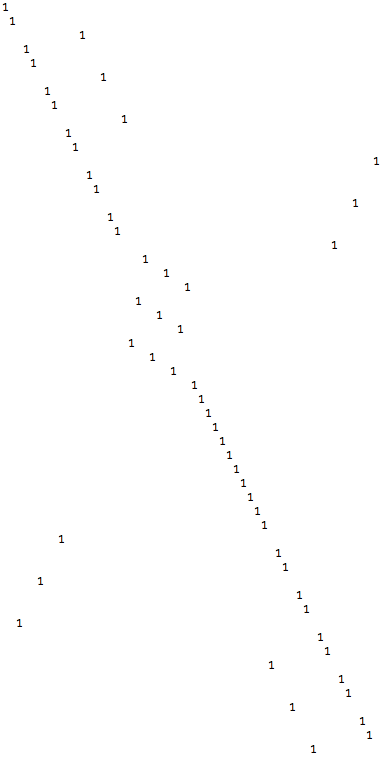
\includegraphics[scale=0.30]{R}
        \caption{R}
    \end{subfigure}
    \hfill
    \begin{subfigure}[h]{0.4 \textwidth}
        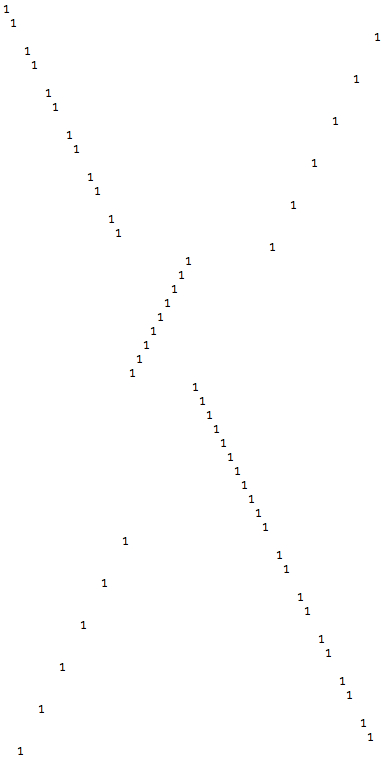
\includegraphics[scale=0.30]{R2}
        \caption{R2}
    \end{subfigure}
    \begin{subfigure}[h]{0.4 \textwidth}
        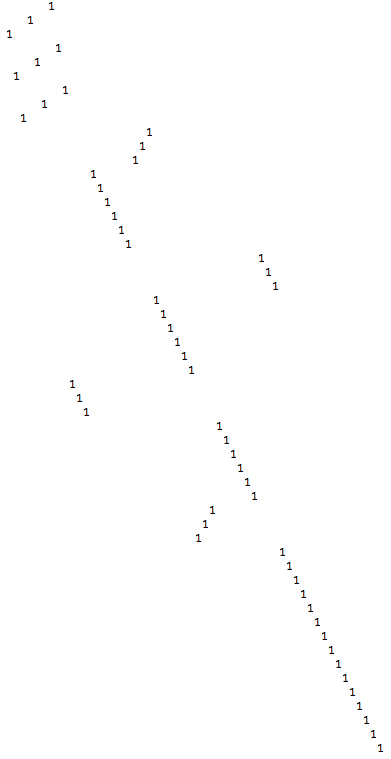
\includegraphics[scale=0.30]{U}
        \caption{U}
    \end{subfigure}
    \hfill
    \begin{subfigure}[h]{0.4 \textwidth}
        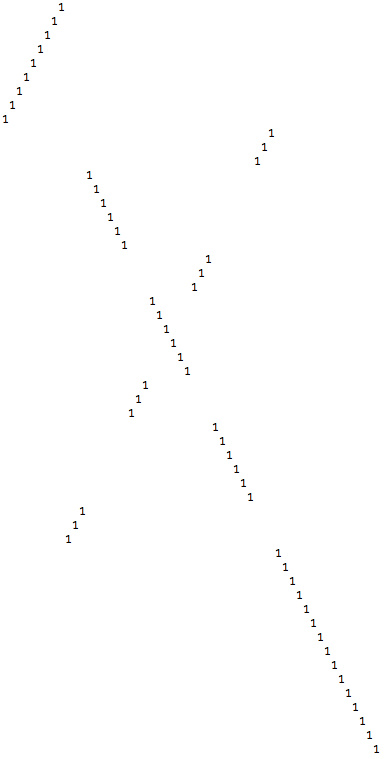
\includegraphics[scale=0.30]{U2}
        \caption{U2}
    \end{subfigure}
    \caption{Matrices for selected standard moves}
\end{figure}

\newpage

\begin{figure}[h!]
  \centering
  \begin{subfigure}[h]{0.4 \textwidth}
      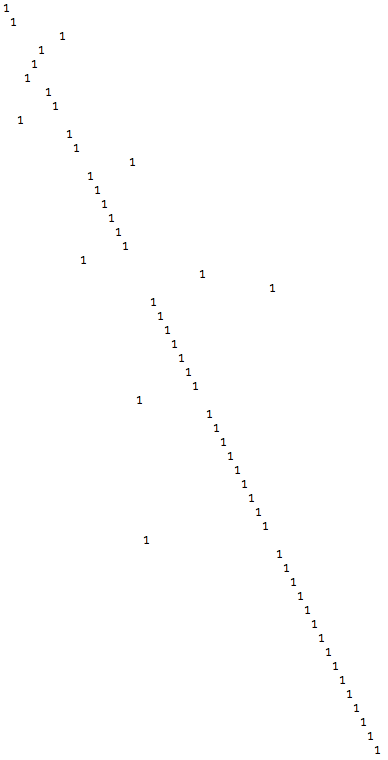
\includegraphics[scale=0.3]{tperm}
      \caption{T-perm}
  \end{subfigure}
  \hfill
  \begin{subfigure}[h]{0.4 \textwidth}
      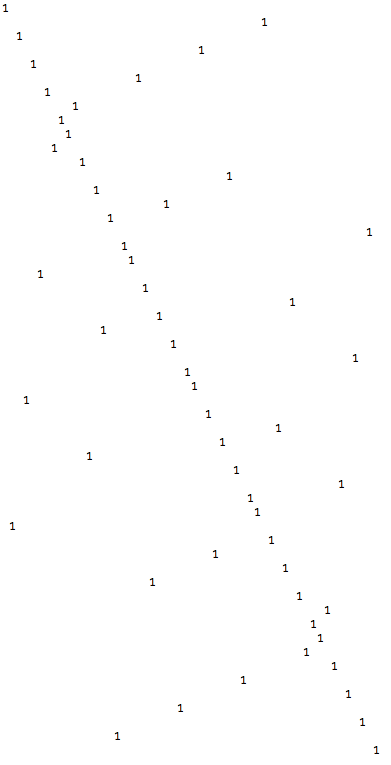
\includegraphics[scale=0.3]{superflip}
      \caption{Superflip}
  \end{subfigure}
  \caption{Matrices for selected algorithms}
\end{figure}

\begin{figure}[h!]
\centering
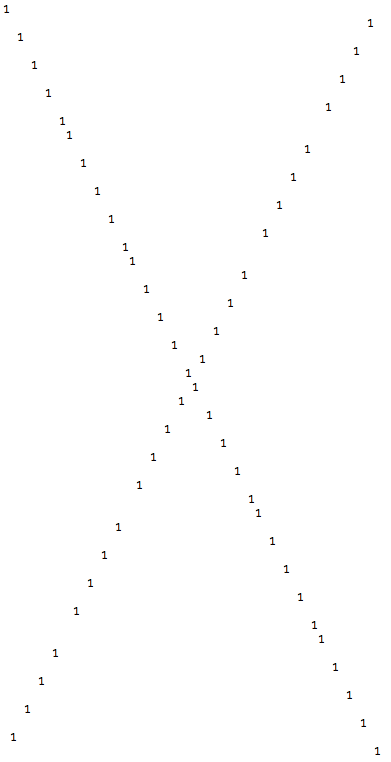
\includegraphics[scale=0.3]{checker}
\caption{Checkerboard}
\end{figure}

Personally, checkerboard is my favorite.

\newpage

\subsection{Miscellaneous Uses}

What state is the cube in after U100000? Since 100000 is divisible by 4, the
cube must be solved. In general, each series of moves has a given ``order'',
the amount of times it can be repeated before the cube is solved again.
One application of matrices is to compute these orders quickly, as matrix
exponentiation can be done quickly with repeated squaring.

\begin{minted}{python}
def mat_exp(A: np.array, k: int) -> list:
    """ Does fast matrix exponentiation """
    v = np.identity(len(A))
    while k > 0:
        if k & 1 == 1:
            v = v @ A
        k >>= 1
        A = A @ A
    return v
\end{minted}

\begin{minted}{python}
# largest group
T = move_mat("R U2 D' B D'")
print(apply(mat_exp(T, 1260), c))

# what's the state after (R U F L B)100000?
T = move_mat("R U F L B")
print(apply(mat_exp(T, 100000), c))
\end{minted}

\section{Mathematical Proofs}

\begin{lemma}
The transpose of a permutation matrix is its inverse.
\end{lemma}

\begin{proof}
By definition of the inverse, \( A A^{-1} = I \).
Thus, it suffices to calculate \( AA^T \).
Think of this product as the sum of the outer products between
each column in \( A \) and each row in \( A^T \).
\[ AA^T = \begin{bmatrix} col_1(A) & col_2(A) & \dots & col_n(A) \end{bmatrix}
\begin{bmatrix} row_1(A^T) \\ row_2(A^T) \\ \dots \\ row_n(A^T) \end{bmatrix} \]
\[ = col_1(A) row_1(A^T) + \dots + col_n(A) row_n(A^T) \]

Each \( col_j(A) row_j(A^T) \) product yields a matrix of all 0's except for
a single 1 at the index where there is a 1 in \( col_j(A) \). Adding them up
yields a matrix which has a 1 on each entry on the diagonal (because each 1
position in the columns of \( A \) is distinct).

Thus, \( col_1(A) row_1(A^T) + \dots + col_n(A) row_n(A^T) = I_n \)
\end{proof}

\begin{corollary}
Because every matrix can be transposed, every permutation matrix is invertible.
\end{corollary}

\newpage

\begin{lemma}
The multiplication of permutation matrices is closed,
that is, for a permutation matrix \( A \) and permutation
matrix \( B \), \( AB \) is a permutation matrix.
\end{lemma}

\begin{proof}
An alternative definition of a permutation matrix is a matrix containing
exactly one entry of 1 in each row and each column and 0s elsewhere.
Multiplying a matrix by a permutation matrix is equivalent to permuting
the rows of the matrix. If the rows are swapped, then they must still
have exactly one 1 in each row. Since swapping rows doesn't change the
number of 1's in each column, each column must also still have exactly
one 1. Thus, the product is a permutation matrix.
\end{proof}

\begin{lemma}
There are a finite number of permutation matrices, namely, there are
\( N! \) permutation matrices for matrices of size \( N \)x\( N \).
\end{lemma}

\begin{proof}
Each permutation matrix is uniquely determined by \( \pi \). There are \(
N! \) possible \( \pi \)'s, so there are \( N! \) permutation matrices.
\end{proof}

\begin{lemma}
\( (P^k)^{-1} = (P^{-1})^k \)
\end{lemma}

\begin{proof}
\begin{align*}
(A_1 A_2 \dots A_n)^{-1} &= A_n^{-1} A_{n - 1}^{-1} \dots A_1^{-1} \\
(P P \dots P)^{-1} &= P^{-1} P^{-1} \dots P^{-1} = (P^{-1})^k
\end{align*}
\end{proof}

\begin{theorem}
For every permutation matrix \( P \), there exists a \( k \) such that \( P^k = I \).
\end{theorem}

\begin{proof}
By lemma 2, each power of \( P \) must be a permutation matrix.
By lemma 3, there are a finite number of permutation matrices, thus
there must be point \( x \) where \( \forall z \geq x \) \( P^z = P^y \)
for some \( y < x \). Picking a particular \( z > x \), if \( P^z = P^y \), then \( P^z (P^y)^{-1} = I \)
so \( P^z (P^{-1})^y = I \), thus \( P^{z - y} = I \), completing the proof.
\end{proof}

\begin{corollary}
Repeating any sequence of moves on a solved Rubik's cube
will bring the cube back to a solved state eventually.
\end{corollary}

\begin{theorem}
The inverse of a series of moves is the series formed
by reversing the original series, inverting each move.
\end{theorem}

\begin{proof}
Let \( S = A_1 A_2 \dots A_n \). \( S^{-1} =  A_n^{-1} A_{n - 1}^{-1} \dots A_1^{-1} \).
\end{proof}

\newpage

\begin{theorem}
NISS. The ``scramble'' and ``solution'' lie in a cycle.
\end{theorem}

\begin{proof}
Proof: Let a scramble be \( ABCD \) and a solution be \( pqrs \).
By the definition of a solution, \( ABCDpqrs = I \).
\( sABCDpqrs = s \) and \( sABCDpqrss^{-1} = ss^{-1} \), so
\( sABCDpqr = I \).
Repeating these operations,
\[ ABCDpqrs = I \]
\[ sABCDpqr = I \]
\[ rsABCDpq = I \]
\[ qrsABCDp = I \]
\[ pqrsABCD = I \]
\[ \dots \]
\end{proof}

Thus, one can either think of the scramble as \( ABCD \) and the solution as
\( pqrs \), or the scramble as \( qrsA \) and the solution as \( BCDp \), or
any variant, so as long the scramble plus the solution is a cyclic rotation
of the original scramble and solution.

\section{Future Work}

Parity derivations, group theory tie-ins, and eigenvalue stuff!
Maybe a faster solving algorithm eventually.

\end{document}
